
\documentclass[border=8pt, multi, tikz]{standalone} 
\usepackage{import}
\subimport{../layers/}{init}
\usetikzlibrary{positioning}
\usetikzlibrary{3d} %for including external image 

\def\ConvColor{rgb:yellow,5;red,2.5;white,5}
\def\ConvReluColor{rgb:yellow,5;red,5;white,5}
\def\PoolColor{rgb:red,1;black,0.3}
\def\UnpoolColor{rgb:blue,2;green,1;black,0.3}
\def\FcColor{rgb:blue,5;red,2.5;white,5}
\def\FcReluColor{rgb:blue,5;red,5;white,4}
\def\SoftmaxColor{rgb:magenta,5;black,7}   
\def\SumColor{rgb:blue,5;green,15}

\newcommand{\copymidarrow}{\tikz \draw[-Stealth,line width=0.8mm,draw={rgb:blue,4;red,1;green,1;black,3}] (-0.3,0) -- ++(0.3,0);}

\begin{document}
\begin{tikzpicture}
\tikzstyle{connection}=[ultra thick,every node/.style={sloped,allow upside down},draw=\edgecolor,opacity=0.7]
\tikzstyle{copyconnection}=[ultra thick,every node/.style={sloped,allow upside down},draw={rgb:blue,4;red,1;green,1;black,3},opacity=0.7]

\tikzset{connection/.style={line width=0.5mm,every node/.style={sloped,allow upside down},draw=\edgecolor,opacity=0.7}}

\node[canvas is zy plane at x=0] (rgb_image) at (2,0,0) {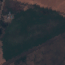
\includegraphics[width=5cm,height=5cm]{../assets/sample_rgb.png}};

\node[canvas is zy plane at x=0] (gndvi_image) at (1,0,0) {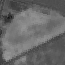
\includegraphics[width=5cm,height=5cm]{../assets/sample_gndvi.png}};

\node[canvas is zy plane at x=0] (ndvi_image) at (0,0,0) {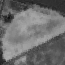
\includegraphics[width=5cm,height=5cm]{../assets/sample_ndvi.png}};

\pic[shift={(0,0,0)}] at (6,0,0) 
    {Box={
        name=convlstm1,
        caption=ConvLSTM Cell 1,
        xlabel={{64, }},
        zlabel=64 x 64,
        fill=\ConvColor,
        height=35,
        width=8,
        depth=35
        }
    };

\draw [connection]  (rgb_image)    -- node {\midarrow} (convlstm1-west);

\pic[shift={(4,0,0)}] at (convlstm1-east) 
    {Box={
        name=convlstm2,
        caption=ConvLSTM Cell 2,
        xlabel={{128, }},
        zlabel=64 x 64,
        fill=\ConvColor,
        height=35,
        width=16,
        depth=35
        }
    };

\draw [connection]  (convlstm1-east)    -- node {\midarrow} (convlstm2-west);

\pic[shift={(4,0,0)}] at (convlstm2-east) 
    {Ball={
        name=gap,
        fill=\SumColor,
        opacity=0.6,
        radius=2.5,
        logo=$+$
        }
    };

\draw [connection]  (convlstm2-east)    -- node {\midarrow} (gap-west);

\pic[shift={(3,0,0)}] at (gap-east) 
    {Box={
        name=fc_logits,
        caption=Logits,
        xlabel={{10, }},
        zlabel=,
        fill=\ConvColor,
        height=25,
        width=1,
        depth=1
        }
    };

\draw [connection]  (gap-east)    -- node {\midarrow} (fc_logits-west);

\end{tikzpicture}
\end{document}
